Bremsstrahlung is emitted, if (high-energetic) charged particles are deflected in an external
electric field, for example the Coulomb field of an atomic nucleus or an shell electron of the
target.
\\
The according Feynman diagrams of lowest order are:
\\
\\
\\
Feynman-Diagramme

\subsubsection*{Energy loss through bremsstrahlung}

For high energies, the loss of energy through bremsstrahlung can be approximated with

\[-\left(\frac{dE}{dx}\right)_{\text{rad}} = 4\alpha \rho N_A \cdot \frac{Z(Z+1)}{A} \cdot z^2\cdot
\left(\frac{1}{4\pi \epsilon_0} \frac{e^2}{mc^2} \right)^2 \cdot E\cdot \text{ln}(183\cdot
Z^{-\frac{1}{3}}) \]

The contribution $Z^2$ is a result of the deflection in the field of the nucleus with the charge
$Z\cdot e$, the one with $Z$ is caused by the deflection in the field of the shell electrons, each
with a charge of $-e$. This does not include that the shell electrons partially shield the nucleus.
Therefore, the formula is only valid for large $E$.
\\
Note: For the second most leightweight particle, the muon, is the loss of energy through
bremsstrahlung already 40,000 times smaller than for the electron.

\[-\left(\frac{dE}{dx}\right)_{\text{rad}} \sim E~~~~~~~~~~\text{und}~~~~~~~~~
-\left(\frac{dE}{dx}\right)_{\text{rad}} \sim \frac{1}{m^2}\]

\subsubsection*{Critical energy $E_c$}

The critical energy is the energy of a projektile where the loss of energy through bremsstrahlung
is equal the loss of energy through the collision:

\[-\left(\frac{dE}{dx}\right)_{\text{rad}} \bigg|_{E_c} = -\left(\frac{dE}{dx}\right)_{\text{coll}}
\bigg|_{E_c}  \]

$E_c$ is dependant of the target material and of the particle type of the projectile (if not
stated otherwise, literature values relate to electrons). The critical energy resizes with about the
square of the mass of the projectile. To obtain the critical energy for muons, for example, we use

\[E_c^\mu = E_c^e \left( \frac{m_\mu}{m_e} \right)^2 \]

There exist different approximations to estimate $E_c$ roughly:

\[E_c = \frac{800}{Z+1{},2}~\text{MeV} \]

or for solids

\[E_c = \frac{610}{Z+1{,}24}~\text{MeV} \]

or for gases

\[E_c = \frac{710}{Z+0{,}92}~\text{MeV} \]

The common values for $E_c$ vary enormously:

\begin{figure}[H]
	\centering
	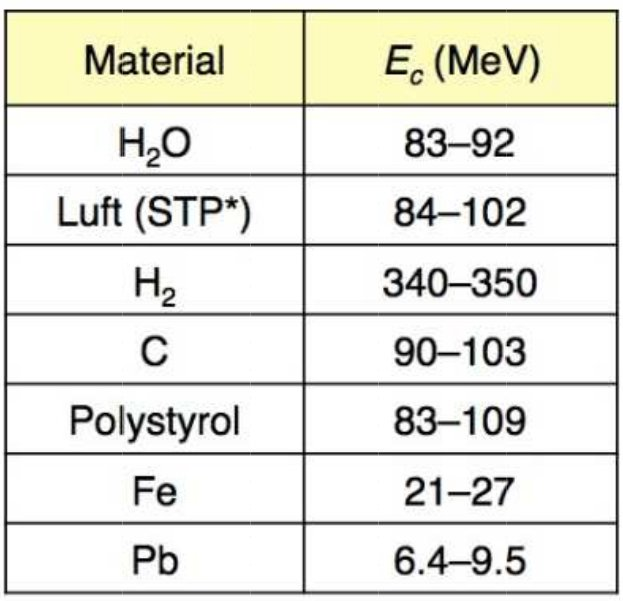
\includegraphics[width=0.5\textwidth]{tabelle1.jpg}
	\caption{}
	\label{}
\end{figure}


\subsubsection*{Radiation length $\chi_0$}


